\documentclass[11pt]{article}

\usepackage[a4paper,margin=1in]{geometry}
\usepackage{array}
\usepackage{booktabs}
\usepackage{enumitem}
\usepackage{graphicx}
\usepackage{tabularx}
\usepackage[hidelinks]{hyperref}
\usepackage{tikz}
\usetikzlibrary{arrows.meta,positioning,fit,shapes.geometric}

\title{IndiciumForge: A Contract-First Open Core for Evidence-First Financial Research Workflows}
\author{Zhengze Yu\thanks{\texttt{cavarad0ssi@outlook.com}}}
\date{July 2026}

\newcommand{\schema}[1]{\texttt{#1}}
\newcommand{\pkg}[1]{\texttt{#1}}
\newcommand{\claim}[1]{\textsuperscript{\textsf{#1}}}
\newcolumntype{Y}{>{\raggedright\arraybackslash}X}

\begin{document}
\maketitle

\begin{abstract}
Financial research pipelines frequently combine data ingestion, proprietary signals,
operator-local state, and implicit execution assumptions in ways that obscure what was
knowable at each staged decision. Migrating away from legacy systems compounds the problem
when teams copy modules instead of preserving observable behavior against frozen references.

IndiciumForge is an open-core Python architecture whose primary outputs are versioned
research artifacts--JSON stage states, CSV review tables, and chain summaries--rather
than orders or portfolio actions. Stable contracts and YAML pack loaders let operator-local
extensions attach without forking core semantics. A manifest audit CLI validates structural
completeness; golden and parity comparators evaluate semantic agreement against exported
reference trees without importing legacy runtime code.

We describe six contributions: contract-first packaging, artifact schema audit,
recipe/session orchestration, an explicit open-core boundary, golden parity methodology,
and agent-friendly governance. A three-layer validation story combines public golden tests,
a synthetic parity demo, and category-level operator sign-off without disclosing private
rows or paths. IndiciumForge is a research audit framework: it is not a trading system, not
investment advice, and not a broker execution platform.
\end{abstract}

\noindent\textbf{Keywords:} research workflows; software architecture; artifact audit;
open core; reproducibility; financial research systems.

\section{Introduction}

Quantitative and fundamental research groups need workflows that support two audit
questions at every stage: what evidence existed at the time, and whether an independent
reviewer can verify that evidence without rerunning hidden state. Execution-optimized stacks
prioritize latency and fill quality; notebook-centric workflows lack schema discipline and
make regressions expensive to detect.

IndiciumForge targets the middle ground: evidence-first financial research implemented as
auditable artifacts behind explicit contracts. The open-source repository ships ports,
schemas, synthetic fixtures, a reference CLI, manifest audit, golden tests, and a parity
harness. Proprietary data adapters, factor detectors, and production recipe bodies remain
in operator-local packs.

\paragraph{Contributions.}
This paper makes six software-architecture contributions:
\begin{enumerate}[leftmargin=*]
  \item Contract-first open core: workflow stages consume port interfaces and pack loaders, not vendor SDKs.\claim{C13-C15}
  \item Artifact schemas and audit CLI: \schema{indiciumforge.*} schema IDs plus structural validation.\claim{C03-C04}
  \item Recipe and session workflow model: cyclic session contracts with domain-specific recipes.\claim{C16-C18}
  \item Open-core/private-extension boundary: an ADR-governed IP and security split.\claim{C12,C29}
  \item Golden artifact and parity methodology: exported references and five parity dimensions.\claim{C05-C11}
  \item Agent-friendly governance: ADRs, agent rules, and in-repository skills for safe automation.\claim{C32-C33}
\end{enumerate}

\paragraph{Non-claims.}
IndiciumForge does not execute live trades or broker orders, provide investment advice,
ship proprietary alpha detectors in the public repository, or claim full replacement of
every legacy workflow surface. Parity \texttt{all\_match} on an operator golden date is
research audit evidence, not production certification.

\section{Problem Statement}

Production research stacks often merge raw and derived data paths, proprietary signal
definitions, local calibration state, and assumptions about session timing or execution
feasibility. When these concerns share one codebase without artifact contracts, reviewers
cannot reconstruct point-in-time evidence. Regression testing devolves into manual diffing
of opaque outputs.

Migration from legacy implementations creates another failure mode: copying modules imports
hidden path assumptions, network side effects, and domain rules that should not become
universal core semantics. This resembles the legacy-code problem of preserving observable
behavior before refactoring, but the preserved surface here is a set of exported research
artifacts rather than in-process APIs \cite{feathers2004legacy}. IndiciumForge compares
artifacts against the frozen reference label \schema{indiciumgrid-golden-v1} and records
behavior outside the covered surface as an intentional change or unsupported gap. Eleven
anti-inheritance rules guard the public core against hidden legacy paths, network fetches,
and direct promotion of raw provider output into strict gate decisions.\claim{C08,C10,C11,C29,C30}

\section{System Architecture}

IndiciumForge v2.0.0 ships three installable packages:
\begin{center}
\begin{tabular}{ll}
\toprule
Package & Responsibility \\
\midrule
\pkg{indiciumforge-core} & Domain models, ports, artifact I/O, manifest audit, parity models \\
\pkg{indiciumforge-workflow} & Market gate kernel, daily review skeleton, workflow chain runner \\
\pkg{indiciumforge-cli} & Typer CLI exposing workflow, artifact, factor, provider, parity commands \\
\bottomrule
\end{tabular}
\end{center}

\begin{figure}[t]
\centering
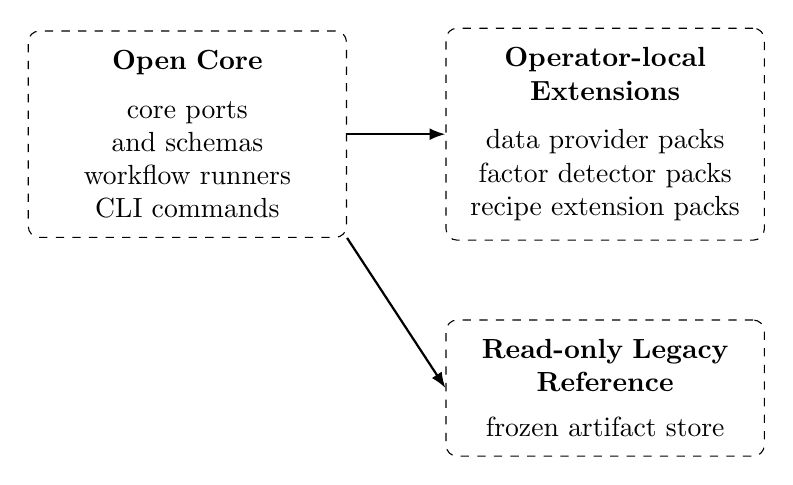
\begin{tikzpicture}[
  boundary/.style={draw, dashed, rounded corners, align=center, inner sep=7pt,
                   text width=3.55cm, minimum height=2.45cm},
  refbox/.style={draw, dashed, rounded corners, align=center, inner sep=7pt,
                 text width=3.55cm, minimum height=1.25cm},
  arrow/.style={-{Latex[length=2mm]}, thick}
]
\node[boundary] (open) {\textbf{Open Core}\\[0.2cm]
  core ports and schemas\\
  workflow runners\\
  CLI commands};
\node[boundary, right=1.25cm of open] (priv) {\textbf{Operator-local Extensions}\\[0.2cm]
  data provider packs\\
  factor detector packs\\
  recipe extension packs};
\node[refbox, below=1.0cm of priv] (ref) {\textbf{Read-only Legacy Reference}\\[0.15cm]
  frozen artifact store};

\draw[arrow] (open.east) -- (priv.west);
\draw[arrow] (open.south east) -- (ref.west);
\end{tikzpicture}
\caption{System boundary. The open core exposes ports and contracts. Operator-local
extensions supply data, factors, and recipe logic. Frozen legacy references support parity
comparison only; they are not imported at runtime.}
\label{fig:boundary}
\end{figure}

\section{Contract-First Design}

Workflow code depends on protocols rather than concrete data vendors. The session-aware
data provider port, factor detector port, and recipe extension port follow the same pack
loading pattern. YAML packs declare \schema{indiciumforge.<type>.v1} schemas and reference
entry-point modules or nested configuration files. Public fixtures demonstrate the mechanism;
operators keep live data adapters and proprietary detectors in private repositories.

Breaking namespace changes bump the major release version. The v2.0.0 rebrand from the
legacy \schema{lucerna.*} namespace includes a one-release compatibility shim that accepts
deprecated IDs with warnings.

\paragraph{Design rationale.}
IndiciumForge does not try to replace a general task scheduler, data lake, or backtesting
engine. Its reusable minimum is narrower: namespaced stage schemas, explicit extension
ports, manifest audit, and parity verdicts for exported reference artifacts. This combination
lets a team keep proprietary adapters and detectors outside the public repository while still
reviewing whether an observable research workflow preserved behavior. In contrast, a generic
DAG can schedule the same stages but does not by itself define the financial-research artifact
contracts or the accepted verdict taxonomy.

\section{Artifact Schema and Manifest Audit}

Each machine-readable artifact carries a \texttt{schema} field using the
\schema{indiciumforge.*} namespace. Stage bundles are stored under predictable directories
such as \texttt{workflows/\{YYYYMMDD\}/<stage>/}. The manifest auditor checks required files,
JSON parseability, expected schema IDs, and trade-date consistency.

\begin{figure}[t]
\centering
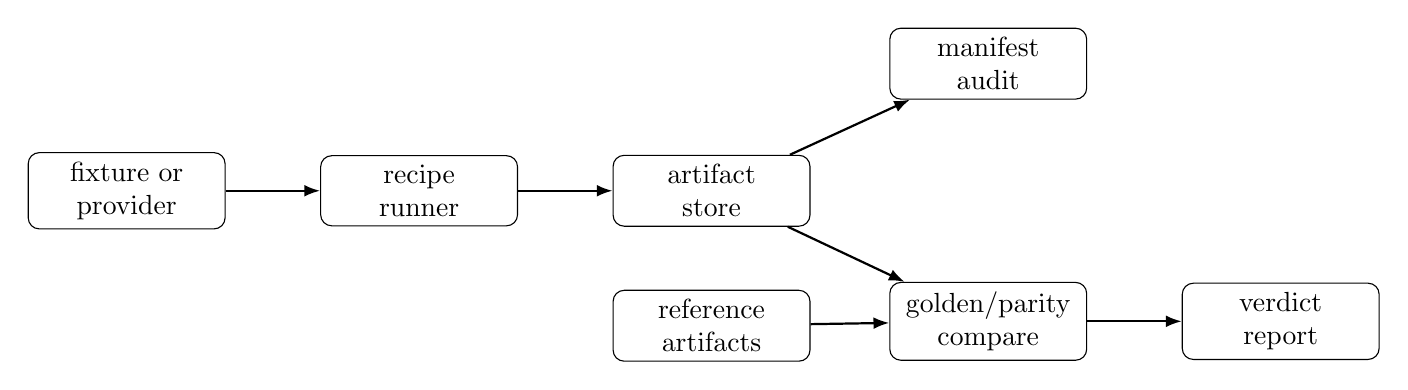
\begin{tikzpicture}[
  node distance=1.1cm and 1.2cm,
  box/.style={draw, rounded corners, align=center, minimum width=2.5cm, minimum height=0.8cm},
  arrow/.style={-{Latex[length=2mm]}, thick}
]
\node[box] (input) {fixture or\\provider};
\node[box, right=of input] (recipe) {recipe\\runner};
\node[box, right=of recipe] (artifacts) {artifact\\store};
\node[box, above right=0.7cm and 1.0cm of artifacts] (audit) {manifest\\audit};
\node[box, below right=0.7cm and 1.0cm of artifacts] (parity) {golden/parity\\compare};
\node[box, right=of parity] (verdict) {verdict\\report};
\node[box, below=0.8cm of artifacts] (ref) {reference\\artifacts};
\draw[arrow] (input) -- (recipe);
\draw[arrow] (recipe) -- (artifacts);
\draw[arrow] (artifacts) -- (audit);
\draw[arrow] (artifacts) -- (parity);
\draw[arrow] (ref) -- (parity);
\draw[arrow] (parity) -- (verdict);
\end{tikzpicture}
\caption{Runtime data flow. Research inputs flow through recipe runners into versioned
artifacts. Manifest audit validates structure; golden and parity comparators evaluate
semantics against reference trees.}
\label{fig:runtime}
\end{figure}

Structural audit is separate from semantic golden comparison. For example, manifest audit can
detect a missing market gate summary before the semantic comparator evaluates strict candidate
sets.

\section{Recipe and Session Model}

IndiciumForge generalizes operator-linear folders into session-cyclic checkpoints linked by
typed handoff artifacts. Core types include asset domains, session models, workflow recipes,
checkpoints, evidence stage references, and handoff artifacts.

The default A-share daily research recipe composes awareness, post-close discovery, preopen
handoff, optional factor scan, and market gate stages. Names such as \texttt{post\_close} are
recipe compatibility labels rather than universal lifecycle enums. Other domains can define
alternate recipes under the same session contracts.

\section{Open-Core / Private-Extension Boundary}

\begin{center}
\begin{tabular}{ll}
\toprule
Open-source repository & Operator-local private packs \\
\midrule
Ports, schemas, loaders & Live data adapters \\
Synthetic fixtures and demo detectors & Proprietary factor logic \\
Recipe runner and extension loader & Production recipe stage implementations \\
Parity harness and synthetic reference demo & Legacy output mirrors, credentials, reference trees \\
\bottomrule
\end{tabular}
\end{center}

This boundary keeps credentials, account identifiers, calibrated policies, and proprietary signal
logic out of the public repository while still enabling real deployments.

\section{Golden Artifact and Parity Methodology}

The public golden layer pins a frozen reference and lists five market-gate scenarios. Public
tests assert semantic agreement with exported expected artifacts. A synthetic parity demo
exercises the same harness without private paths.

\begin{table}[t]
\centering
\small
\begin{tabularx}{\linewidth}{lYl}
\toprule
Evidence layer & Public or reported evidence & Claim IDs \\
\midrule
Package surface & Three installable packages and the \texttt{indiciumforge} CLI & C01, C02 \\
Static and unit gates & Ruff in CI; pytest reported 144 passed and 1 skipped at draft time & C19, C20 \\
Golden market gate & Five exported market-gate scenarios under \schema{indiciumgrid-golden-v1} & C05, C10 \\
Synthetic parity & Public \texttt{parity\_reference\_demo} exercises the harness without private paths & C09, C22 \\
Governance & 23 ADRs plus anti-inheritance rules and agent onboarding documents & C29, C32, C33 \\
\bottomrule
\end{tabularx}
\caption{Artifact-based evidence used in this paper. The table reports software and
audit evidence only; it does not report trading performance, investment recommendations, or
broker execution results.}
\label{tab:evidence}
\end{table}

\begin{figure}[t]
\centering
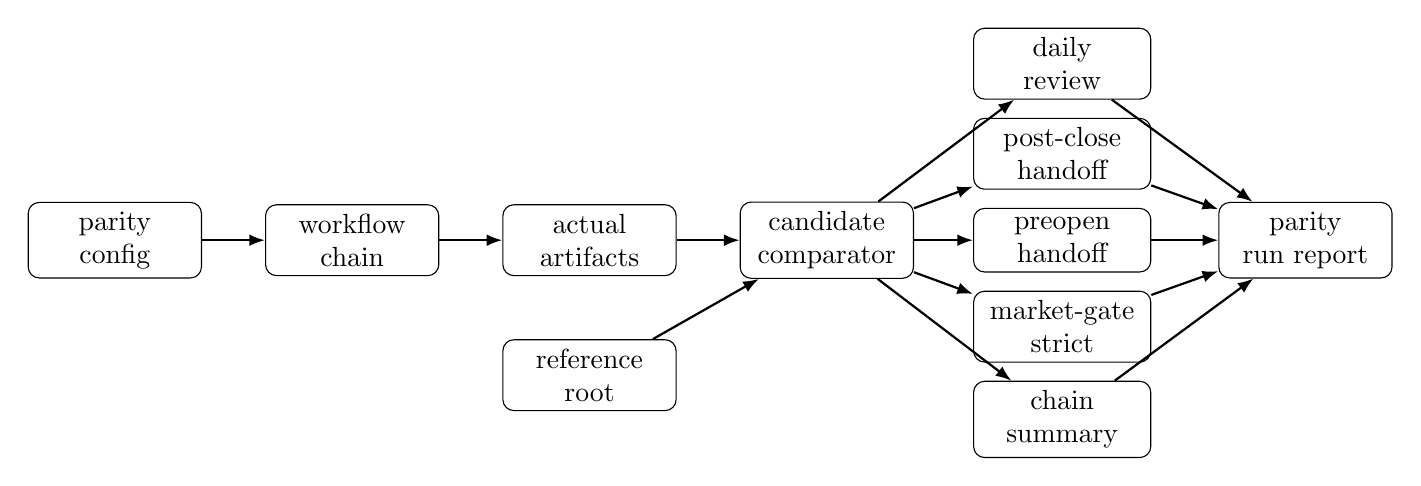
\begin{tikzpicture}[
  node distance=0.8cm and 0.8cm,
  box/.style={draw, rounded corners, align=center, minimum width=2.2cm, minimum height=0.72cm},
  small/.style={draw, rounded corners, align=center, minimum width=2.25cm, minimum height=0.62cm},
  arrow/.style={-{Latex[length=2mm]}, thick}
]
\node[box] (config) {parity\\config};
\node[box, right=of config] (runner) {workflow\\chain};
\node[box, right=of runner] (actual) {actual\\artifacts};
\node[box, below=of actual] (ref) {reference\\root};
\node[box, right=of actual] (cmp) {candidate\\comparator};
\node[small, right=0.75cm of cmp] (d3) {preopen\\handoff};
\node[small, above=0.23cm of d3] (d2) {post-close\\handoff};
\node[small, above=0.23cm of d2] (d1) {daily\\review};
\node[small, below=0.23cm of d3] (d4) {market-gate\\strict};
\node[small, below=0.23cm of d4] (d5) {chain\\summary};
\node[box, right=0.85cm of d3] (report) {parity\\run report};
\draw[arrow] (config) -- (runner);
\draw[arrow] (runner) -- (actual);
\draw[arrow] (actual) -- (cmp);
\draw[arrow] (ref) -- (cmp);
\draw[arrow] (cmp) -- (d1);
\draw[arrow] (cmp) -- (d2);
\draw[arrow] (cmp) -- (d3);
\draw[arrow] (cmp) -- (d4);
\draw[arrow] (cmp) -- (d5);
\draw[arrow] (d1) -- (report);
\draw[arrow] (d2) -- (report);
\draw[arrow] (d3) -- (report);
\draw[arrow] (d4) -- (report);
\draw[arrow] (d5) -- (report);
\end{tikzpicture}
\caption{Artifact parity flow. The harness runs a recipe chain into an artifact root, compares
five configured dimensions against a reference root, and emits a parity report with
per-dimension verdicts.}
\label{fig:parity}
\end{figure}

The parity harness evaluates daily review structure, post-close handoff shape, preopen
handoff shape, market-gate strict semantics, and workflow chain summary fields. Reports carry
a research-audit disclaimer. Historical \schema{indiciumgrid.*} IDs remain only in frozen
golden expected artifacts.

\section{Case Study: Migration Evidence Without Private Data}

The validation story is intentionally layered. Layer L1 uses public golden market-gate tests,
including strict-pass evidence. Layer L2 uses a synthetic parity demo. Layer L3 is an
operator-local sign-off summarized only at category level. No private paths, tickers, row-level
data, or trading performance appear in this section.

\begin{table}[t]
\centering
\small
\begin{tabularx}{\linewidth}{lY}
\toprule
Layer & Evidence summary \\
\midrule
L1: OSS golden & Five public market-gate scenarios exercise strict, observation, watch, and rejected bucket semantics. The public golden layer includes strict-pass evidence. \\
L2: synthetic parity & The public parity demo exercises the harness path and includes strict-count evidence without private paths. \\
L3: operator sign-off & On golden date \texttt{2026-07-03}, five of five parity dimensions matched and the aggregate verdict was \texttt{all\_match: true}. No mismatch was attributed to an IndiciumForge open-core bug or private extension defect. \\
\bottomrule
\end{tabularx}
\caption{Three-layer migration evidence. L1 and L2 are public and reproducible; L3 is
reported only as category-level sign-off to preserve the private-extension boundary.}
\label{tab:case-layers}
\end{table}

The L3 golden date covered the dimensions shown in Table~\ref{tab:l3-dimensions}. Two other
candidate dates were intentionally classified as unsupported gaps rather than failures: the
\texttt{2026-06-24} frozen reference layout lacked the stage directory needed for parity
prepare, and the \texttt{2026-06-23} legacy post-close layout lacked the required handoff
artifact. These blocked dates document reference coverage limits, not open-core defects.

\begin{table}[t]
\centering
\small
\begin{tabularx}{\linewidth}{lY}
\toprule
Parity dimension & Golden-date category verdict \\
\midrule
\texttt{daily\_review\_structure} & match \\
\texttt{post\_close\_handoff\_shape} & match \\
\texttt{preopen\_handoff\_shape} & match \\
\texttt{market\_gate\_strict\_semantics} & match \\
\texttt{workflow\_chain\_summary\_v4} & match \\
\bottomrule
\end{tabularx}
\caption{Category-level L3 verdicts for golden date \texttt{2026-07-03}. The table mirrors
the reconciled v1.0-rc1 evidence summary without disclosing private artifacts.}
\label{tab:l3-dimensions}
\end{table}

The frozen operator reference contains no \texttt{strict\_count > 0} date. Strict-pass
semantics are therefore supported by L1 public golden scenarios and L2 synthetic parity rather
than by the private frozen-reference export. This distinction prevents the case study from
over-claiming production coverage while preserving the useful behavioral migration evidence.

\section{Availability and Governance}

IndiciumForge ships agent-facing guidance alongside human documentation: AGENTS.md,
architecture decision records, onboarding maps, and in-repository skills for orientation,
extension authoring, and release audit. These documents encode what automation must not do:
inherit legacy paths, publish private data, or treat research artifacts as execution signals.
The source repository is publicly available under the Apache-2.0 license, with package
publication and MCP/plugin surfaces documented as future operational work.

\section{Reproducibility}

From a clean checkout of tag \texttt{v2.0.0}:
\begin{verbatim}
pip install -e packages/indiciumforge-core \
            -e packages/indiciumforge-workflow \
            -e packages/indiciumforge-cli \
            -e ".[dev]"
python -m ruff check .
python -m pytest -q
indiciumforge parity run \
  --parity-config tests/fixtures/parity_reference_demo/parity_config_demo.yaml \
  --artifact-root /tmp/indiciumforge-parity-demo
\end{verbatim}
At draft time the public suite reported 144 passing tests and one skipped test. The parity
command emits a \texttt{parity\_run\_report.json} with dimension-level verdicts.

\section{Limitations and Threats to Validity}

IndiciumForge is not a trading system, investment adviser, or broker execution platform. Public
workflows use synthetic fixtures by default. Manifest audit proves structural completeness, not
economic correctness. The public repository does not include proprietary detectors, private
reference trees, account artifacts, or live provider credentials. Operator-local L3 evidence is
self-reported at category level; it is useful for migration sign-off but is not a third-party
replication. Accounting-risk anomaly detection is future work only.

\section{Related Work}

IndiciumForge sits between several families of tools. Workflow systems such as Apache Airflow
\cite{airflowdocs} and Snakemake \cite{koster2012snakemake} provide scheduling and dependency
management. Experiment and data tools such as MLflow \cite{mlflow2018}, DVC
\cite{dvcdocs}, and Great Expectations \cite{greatexpectationsdocs} help track runs, data
versions, or data quality. Trading and research stacks such as Zipline \cite{ziplinedocs},
Backtrader \cite{backtraderdocs}, and Qlib \cite{qlib2020} focus on backtesting, strategy
research, or quantitative investment workflows. Provenance standards such as W3C PROV
\cite{provdm} provide a broader model for representing entities, activities, and agents.
Software-engineering work on legacy code and technical debt motivates IndiciumForge's
emphasis on characterization evidence and explicit system boundaries \cite{feathers2004legacy,sculley2015hidden}.

\begin{table}[t]
\centering
\small
\begin{tabularx}{\linewidth}{lYYY}
\toprule
Family & Primary output & Typical strength & IndiciumForge contrast \\
\midrule
Workflow schedulers & Task runs and DAG state & Scheduling and retries & Stage artifacts and parity verdicts are first-class \\
Data/experiment tools & Versioned data, metrics, expectations & Dataset and run management & Multi-file financial-research bundles and manifest audit \\
Backtest/trading frameworks & Returns, orders, positions, simulations & Strategy evaluation & Broker execution and advice are out of scope \\
Provenance standards & General provenance graphs & Interoperable provenance model & Lightweight local audit via schema IDs and stage states \\
\bottomrule
\end{tabularx}
\caption{Positioning against adjacent tool families. IndiciumForge is not a general
scheduler, data-versioning system, or backtesting engine; its contribution is the combination
of financial-research artifact contracts, open-core extension boundaries, and parity evidence.}
\label{tab:related}
\end{table}

Its evaluation is artifact-based: tests, golden scenarios, parity reports, ADRs, and
boundary-preserving migration evidence. This differs from benchmark-oriented toolbox papers:
IndiciumForge does not claim model accuracy, trading performance, or benchmark-style
leaderboard results.

\section{AI Assistance Disclosure}

Drafting and repository-maintenance workflows used AI coding assistants, including Cursor and
Codex, to generate draft text, LaTeX conversions, diagrams, and audit prompts. Human review
retained responsibility for claim selection, private-boundary enforcement, citation curation,
and final submission decisions. The claims register is used as a guard against unsupported
technical statements.

\section{Future Work}

Future work includes point-in-time accounting-risk anomaly detection, research dossier
contracts, MCP tools for manifest and parity inspection, IDE plugin packaging of agent skills,
and additional domain recipes. These directions should retain the research-audit boundary and
avoid embedding competition- or broker-specific execution paths into the open core.

\section{Conclusion}

IndiciumForge shows that financial research workflows can be restructured around auditable
artifacts and explicit contracts, enabling legacy migration evidence through golden and parity
methodology rather than module inheritance. The architecture prioritizes reviewer trust and
reproducible stage evidence over execution latency, making it appropriate for research audit
rather than broker routing.

\bibliographystyle{plain}
\bibliography{references}

\end{document}
